\section{Domain decomposition}
% * <felipe.cruz.v@gmail.com> 2018-06-04T10:33:10.994Z:
% 
% > Domain decomposition
% I think you need a high level explanation before jumping into the details, otherwise you would have to read the whole section to infer what is going on. I.e.:
% Can you explain at the start of this section what is the objective of the domain decomposition from a very abstract point of view (e.g. distribute partitions of the domain among multiple compute nodes)? and how it achieves the goal with pseudo code:
% * what are the inputs
% * how that inputs if transformed into subdivision
% * how the models for the compute and communication for each cell is built
% *how the optimization is run to load balance
% * what is the output
% 
% ^.
Domain decomposition in the context of this thesis refers to the process of dividing a computational domain into smaller parts in order to run on multiple processing units.
Importantly, domain decomposition in this context is not be confused with the \textit{domain decomposition method} in mathematics and numerical analysis.
The \textit{domain decomposition method} is used to solve boundary value problems by splitting them into smaller parts.
Instead, domain decomposition in high performance computing and this thesis is the name of the process used to prepare a domain for distribution to multiple processing units.
Specifically, domain decomposition in this thesis is used for solving partial differential equations using finite difference methods on multiple processing units.

The next sections outline the general approach to domain decomposition, the specifics of the model developed and used in this thesis, an overview of the graph partitioning method, and an example for the subdivision model and graph partitioning for domain decomposition.

\subsection{General approach}
Some form of domain decomposition is necessary for any distributed computation.
However, the process of decomposing a domain can vary widely depending on the problem that is distributed i.e. the domain.

Many domain decomposition approaches have some overlap with load balancing approaches. 
For example, many approaches for both work by over-decomposing the domain into more parts than processing units.
This over-decomposing allows in a second step to distribute the smaller parts to the processing units in a smart way to minimize a given set of cost factors.

For domain decomposition the two main cost factors are distributing the same number of grid points to each processing i.e. \textbf{computational cost} and minimizing the amount of communication between different processing units i.e. \textbf{communication cost}.

Given these smaller domain parts and their corresponding cost factors a graph partitioning algorithm can be applied to get a balanced distribution for each processing unit.

This two step process describes the general approach to domain decomposition and is described in more detail as pseudo-code in algorithm \ref{alg:domaindecomposition}.

To note in algorithm \ref{alg:domaindecomposition} is that the over-decomposition method introduces one new parameter: the number of subdivisions per dimension.
This parameter is further explained in section \ref{sec:subdivmodel}.

\begin{algorithm}[!htbp]
\SetKwProg{Fn}{Function}{}{}
\SetKwProg{Ds}{Datastructure}{}{}
\SetKwFunction{SubdivideDomain}{SubdivideDomain}
\SetKwFunction{GraphPartitioning}{GraphPartitioning}
\SetKwFunction{stores}{Stores}
\SetKwFunction{StoreSubdivisionInformation}{StoreSubdivisionInformation}
\KwIn{Computational Domain, Number of Processing Units, Stencil Information}
\KwOut{Decomposed Domain, Partitioning for each Processing Unit}
\BlankLine
\Ds{DomainSubdivision}{
\stores$\left(id, size, boundaries, gridpoints, neighbors\right)$
}
\BlankLine
\Fn{DomainDecomposition(Domain, NumProcs, StencilExtent)}{
\tcc{Step 1: Over-decompose domain and store subdivisions in adjacency list.}
\\
SubdivisionWeightedAdjacencyList, ListOfDomainSubdivisions $\leftarrow$ 
\SubdivideDomain{Domain(SizePerDim, PeriodicityPerDim), NumSubdivPerDim, StencilExtent}
\\
\tcc{Step 2: Partition subdivisions based on adjacency list.}
\\
PartitionList $\leftarrow$ \GraphPartitioning{SubdivisionWeightedAdjacencyList, NumProcs}
}
\BlankLine

\Fn{SubdivideDomain(SizePerDim, PeriodicityPerDim, NumSubdivPerDim, StencilExtent)}{
\tcc{Calculate derived information:}
\\
TotalNumberOfSubdivisions $\leftarrow$ NumSubdivPerDim
\\
SizeOfSubdivision $\leftarrow$ Domain, NumSubdivPerDim
\\
SizeOfBoundaries $\leftarrow$ SizeOfSubdivision, StencilExtent
\\
\tcc{Create adjacency list:}
\\
\ForEach{Subdivision in TotalNumberOfSubdivisions}{
    \ForEach{Direction}{
        Neighbors $\leftarrow$ HandleDomainBoundaries$\left(NumSubdivPerDim, PeriodicityPerDim\right)$
        }

    AppendToWeightedAdjacencyList $\leftarrow$ Neighbors, SizeOfSubdivision, SizeOfBoundaries
\\
    \StoreSubdivisionInformation{id, size, boundaries, gridpoints, neighbors}
}
\Return SubdivisionWeightedAdjacencyList, ListOfDomainSubdivisions
}
\BlankLine
\Fn{GraphPartitioning(SubdivisionWeightedAdjacencyList, NumProcs)}{
\If{FileOutputIsEnabled}{
WriteAdjacancyListToFile(SubdivisionWeightedAdjacencyList, FormatFlag)
}
CallGraphPartitioningLibrary(SubdivisionWeightedAdjacencyList, NumProcs)
\\
\Return Partitioning
}
\BlankLine
\caption{Pseudo-code description of the two-step process to decompose a domain.}
\label{alg:domaindecomposition}
\end{algorithm}

The flowchart in figure \ref{fig:library_flowchart} gives a more abstract overview of the whole automatic domain decomposition process.

\begin{figure}
\centering
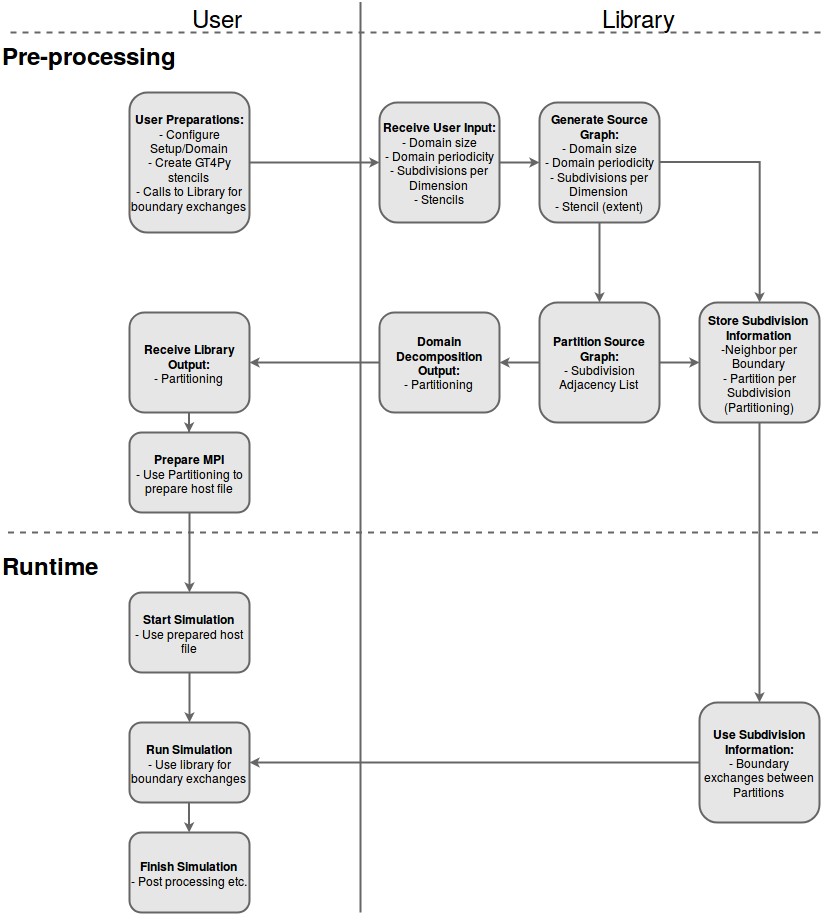
\includegraphics[width=\textwidth]{ddflowchart.png}
\caption{Schematic description of the flow for the automatic domain decomposition process.}
\label{fig:library_flowchart}
\end{figure}

\subsection{Subdivision model for source graph generation}
\label{sec:subdivmodel}
As mentioned before source graphs where every source graph node represents a single physical domain grid point would be impractical for large domains.
Therefore, any alternative has to combine some of these domain grid points into separate divisions even before the domain decomposition occurs.

%TODO
A model to simplify the source graph generation should 

\paragraph{The simplest method}of subdividing a regular grid is by splitting it across each dimension separately, i.e. creating a number of uniform subdivisions.

This guarantees that every subdivision has the same amount of neighbors, with the exception of sections at the boundary of the physical domain if the boundary is not periodic.
Also every subdivision has the same size and therefore distributing them equally during the graph partitioning also means distributing the grid points equally.

For this kind of subdivisions it is simple to define the interior and boundary between subdivisions, as visualized for a two-dimensional and three-dimensional example in fig. \ref{fig:2D_subdivision} and fig. \ref{fig:3D_subdivision} respectively.
This distinction is important for the calculations of the communication and computational cost as described in sections \ref{sec:commcost} and \ref{sec:compcost}.

One limit to the minimal size of a subdivision in any direction is given by the corresponding stencil extend.
Meaning a stencil can not extend into multiple subdivisions, but only the direct neighbor, otherwise subdivision would have multiple neighbors in the same direction.
This should not be a problem, since usually stencils are not as large as any reasonable sized subdivision.

\begin{figure}[!htbp]
\centering
\begin{subfigure}{0.8\textwidth}
  \centering
  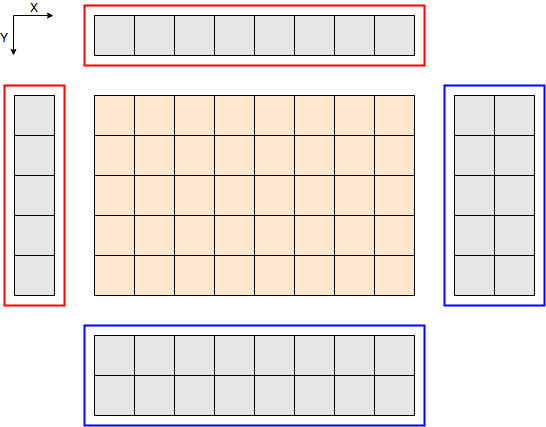
\includegraphics[width=0.9\linewidth]{2D_Block.png}
  \caption{In the middle and in light red the grid points belonging to this subdivision.
Outside in gray the four halo regions.
The red and blue lines surrounding the halo region indicates negative and positive directions respectively.}
  \label{fig:2DBlock}
\end{subfigure}%
\begin{subfigure}{0.2\textwidth}
  \centering
  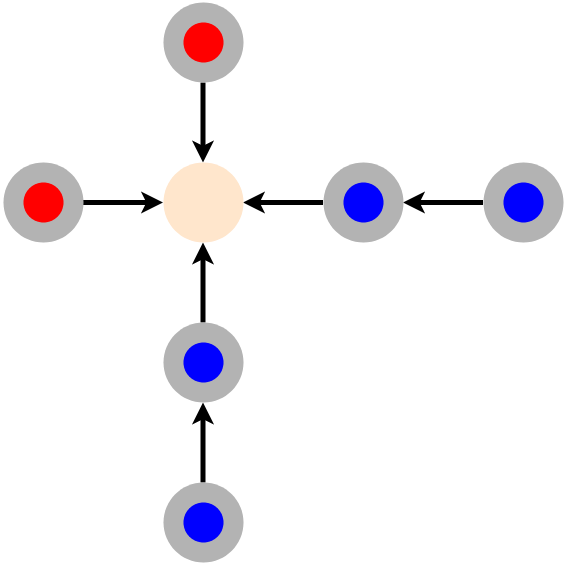
\includegraphics[width=0.9\linewidth]{2D_Block_stencil.png}
  \caption{Stencil representation corresponding to the subdivision in figure \ref{fig:2DBlock}.}
  \label{fig:2DBlockStencil}
\end{subfigure}
\caption{Schematic view of a single two-dimensional domain subdivision.}
\label{fig:2D_subdivision}
\end{figure}

\begin{figure}[!htbp]
\centering
\begin{subfigure}{0.8\textwidth}
  \centering
  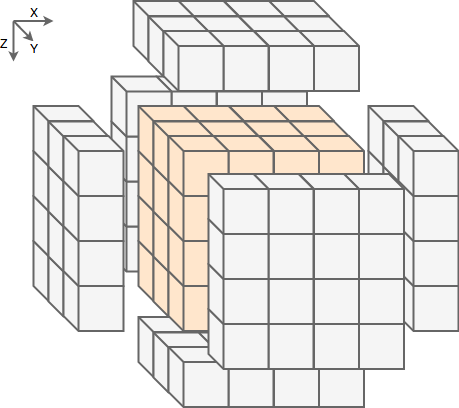
\includegraphics[width=0.9\linewidth]{3D_Block.png}
  \caption{In the middle and in light red the grid points belonging to this subdivision.
Outside in gray the six halo regions.}
  \label{fig:3DBlock}
\end{subfigure}%
\begin{subfigure}{0.2\textwidth}
  \centering
  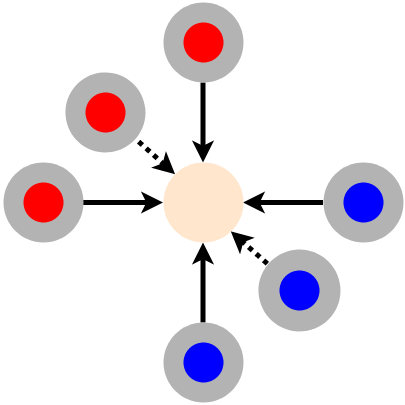
\includegraphics[width=0.9\linewidth]{3D_Block_stencil.png}
  \caption{Stencil representation corresponding to the subdivision in figure \ref{fig:3DBlock}.}
  \label{fig:3DBlockStencil}
\end{subfigure}
\caption{Schematic view of a single three-dimensional domain subdivision.}
\label{fig:3D_subdivision}
\end{figure}

\subsubsection{Communication cost}
\label{sec:commcost}
The communication cost between subdivisions is the main criteria being minimized in the graph partitioning algorithm.
Splitting the domain into uniform subdivisions keeps the communication cost computation simple.

The communication cost for each neighbor of the subdivision is determined by the size of the boundary between the two and the extent of the stencil in the corresponding direction.

For three dimensional domains the communication cost can therefore be computed from the following formula:
\begin{equation}
cc\left(i\right) = sds\left(\left(\floor[\Big]{\frac{i}{2}} - 1\right) \% 3 \right) \cdot sds\left(\left(\floor[\Big]{\frac{i}{2}} + 1\right) \% 3 \right) \cdot se\left(i\right)
\end{equation}
where $cc\left(i\right)$ is the communication cost for side $i$.
The index $i \in \left[0, 1, 2, 3, 4, 5\right]$ is combination of side and dimension, i.e. $0$ is negative x direction, $1$ is positive x-direction, $2$ is negative y-direction and so on.
$sds\left(j\right)$ is the subdivision size of dimension $j \in \left[0,1,2\right]$.
Lastly $se\left(i\right)$ is the stencil extend of side and dimension $i$.
The division, rounding and modulo in the formula is simply a short version of selecting the index of the other two dimensions for the computation of the area between two subdivisions.

\subsubsection{Computational cost}
\label{sec:compcost}
The computational cost, corresponding also to the vertex weight in the source graph, is even easier to compute, since it is proportional to the number of grid points inside the subdivision.

\subsection{Load balancing - graph partitioning method}

Figure \ref{fig:sourcegraph} shows three possible partitions for an example source graph.
For visual simplicity a two-dimensional domain is used, however a three-dimensional domain would work in the same way.
The source graph corresponds to a domain of size $30 \times 40$ with three subdivisions in x-direction and two subdivisions in y-direction.
In this example these six subdivisions are partitioned to two partitions, represented by the color of the circle in the figures \ref{fig:cut1}, \ref{fig:cut2}, and \ref{fig:cut3}.

Figure \ref{fig:cut1} shows a case where a graph partitioning cut causes a computational imbalance between the partitions.
Partitioning one subdivision more to one partition in such a small example causes a very large imbalance.
Usually the graph partitioning method would not allow a result with this much imbalance.
However, in larger graphs some computational imbalance up to a threshold is very common.
Most graph partitioning methods allow manipulating the imbalance threshold.

The mixed direction cut shown in fig. \ref{fig:cut2} has the largest communication cost of the three partitions shown here.
However, it is a fully valid partition and partition boundaries that look similar are common in partitioning of larger graphs.
See the boundary between the brown and red partition in fig. \ref{fig:metis1} for example.
This should highlight the importance of having defined clear and simple defined boundaries in the subdivision model, since the graph partitioning model already adds complexity to the partition boundaries.

Finally, fig. \ref{fig:cut3} shows the ideal case for this small example.
Ideal cuts like this are only likely in such small and simple cases.

\begin{figure}[!htbp]
\begin{subfigure}{0.34\textwidth}
%  \centering
  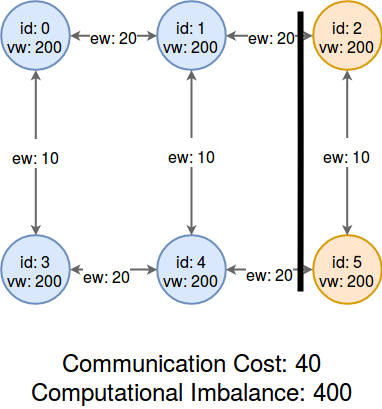
\includegraphics[width=0.95\linewidth]{source_graph_cut3.png}
  \caption{X-direction cut.}
  \label{fig:cut1}
\end{subfigure}%
\begin{subfigure}{0.34\textwidth}
%  \centering
  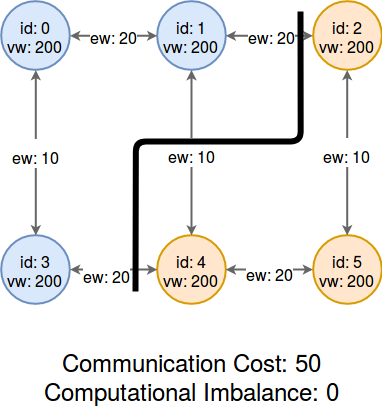
\includegraphics[width=0.95\linewidth]{source_graph_cut2.png}
  \caption{Mixed direction cut.}
  \label{fig:cut2}
\end{subfigure}%
\begin{subfigure}{0.34\textwidth}
%  \centering
  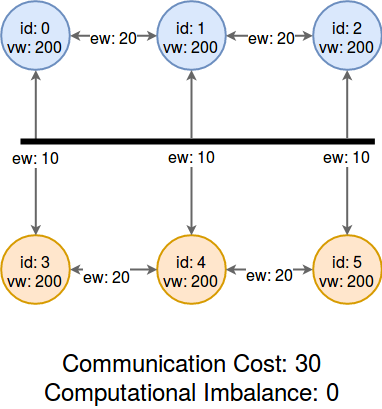
\includegraphics[width=0.95\linewidth]{source_graph_cut1.png}
  \caption{Y-direction cut.}
  \label{fig:cut3}
\end{subfigure}\hfill
\caption{Visual representation for a small graph partitioning example.
Each circle represents one subdivision of size $10 \times 20$.
The label "id" is the subdivision identification number.
The label "vw" describes the vertex weight and is equal to the size of the subdivision.
The label "ew" describes the edge weight and is equal to the size of the boundary between the corresponding subdivisions.
The color of the circle depicts the corresponding partition.
The thick, black line shows the boundary between the two partitions i.e. the cut chosen by the graph partitioning.}
\label{fig:sourcegraph}
\end{figure}

\subsection{Example subdivision and domain decomposition}
The following example should highlight some aspects of the discussed subdivision and domain decomposition.

All the following figures in this section use the same domain and stencil.
The domain has size $2048 \times 1024 \times 40$ and the stencil extends are given as $\left[1, 1, 1, 1, 0, 0\right]$.
This means the stencil uses $1$ neighboring grid point in negative and positive x- and y-direction.
The boundary of the domain is also periodic in x-direction and non-periodic in y- and z- direction.

The figures \ref{fig:metis1}, \ref{fig:pymetis1}, and \ref{fig:scotch1} show the results if the domain is split into $16 \times 8 \times 1$ subdivisions.
This means every box in the figures represents $128 \times 128 \times 40$ grid points.

For comparison the figures \ref{fig:metis2}, \ref{fig:pymetis2}, and \ref{fig:scotch2} show the results if the domain is split into $32 \times 16 \times 1$ subdivisions.
This means every box in the figures represents $32 \times 32 \times 40$ grid points and 4 of these boxes correspond to one box in the figures on the left side.

This comparison should highlight the difference the number of subdivisions and their size can make for the overall domain decomposition.
Also the difference the graph partitioning can make is shown in fig. \ref{fig:rectangular1}.


\begin{figure}[!htbp]
\centering
\begin{subfigure}{0.5\textwidth}
  \centering
  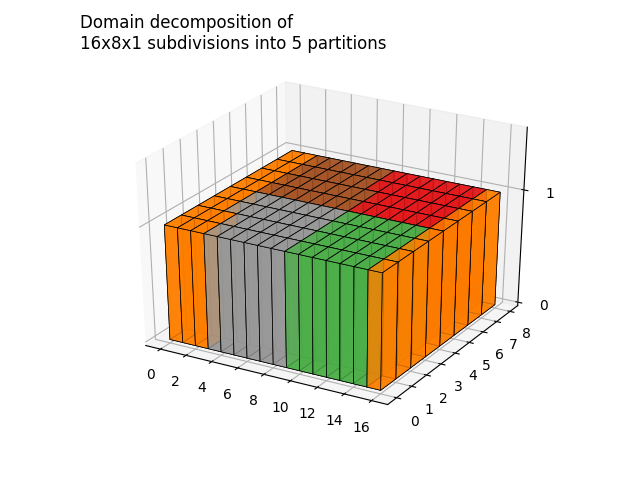
\includegraphics[width=0.9\linewidth]{metis16Px8x1.png}
  \caption{Partitioned by Metis.}
  \label{fig:metis1}
\end{subfigure}%
\begin{subfigure}{0.5\textwidth}
  \centering
  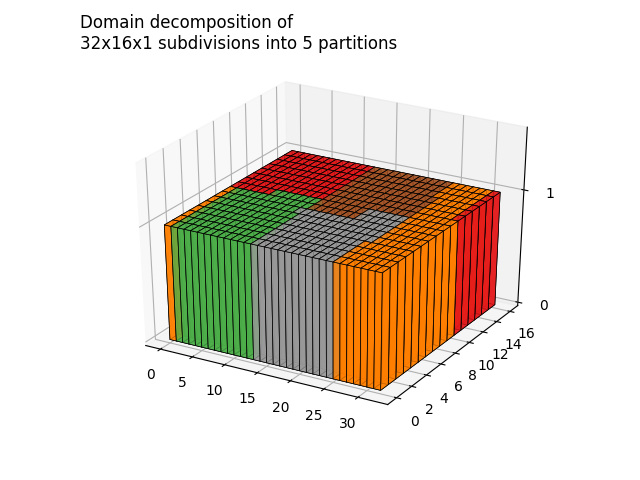
\includegraphics[width=0.9\linewidth]{metis32Px16x1.png}
  \caption{Partitioned by Metis.}
  \label{fig:metis2}
\end{subfigure}

\begin{subfigure}{0.5\textwidth}
  \centering
  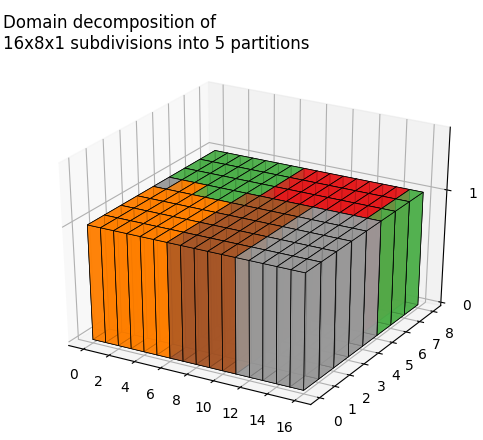
\includegraphics[width=0.9\linewidth]{pymetis16Px8x1.png}
  \caption{Partitioned by PyMetis}
  \label{fig:pymetis1}
\end{subfigure}%
\begin{subfigure}{0.5\textwidth}
  \centering
  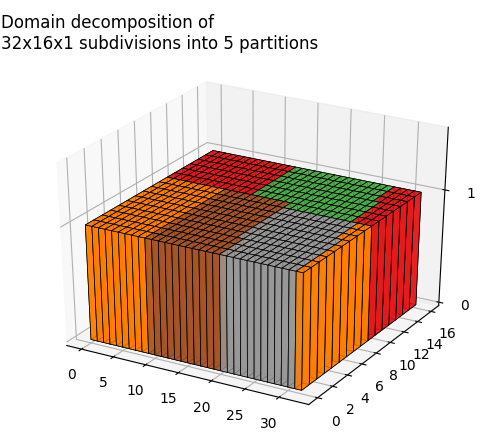
\includegraphics[width=0.9\linewidth]{pymetis32Px16x1.png}
  \caption{Partitioned by PyMetis}
  \label{fig:pymetis2}
\end{subfigure}

\begin{subfigure}{0.5\textwidth}
  \centering
  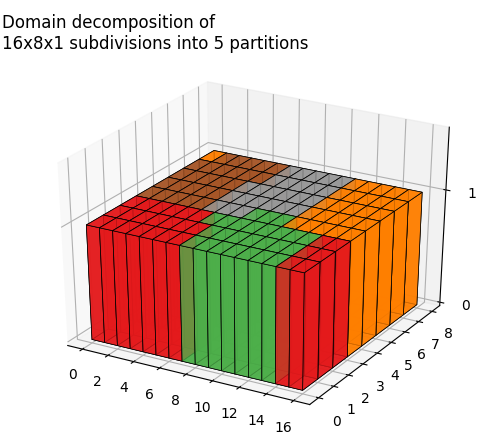
\includegraphics[width=0.9\linewidth]{scotch16Px8x1.png}
  \caption{Partitioned by Scotch}
  \label{fig:scotch1}
\end{subfigure}%
\begin{subfigure}{0.5\textwidth}
  \centering
  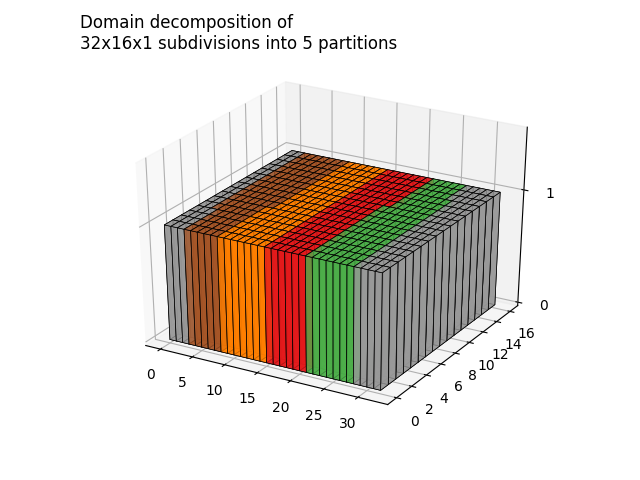
\includegraphics[width=0.9\linewidth]{scotch32Px16x1.png}
  \caption{Partitioned by Scotch}
  \label{fig:scotch2}
\end{subfigure}

\caption{Domain subdivision and domain decomposition into 5 partitions. 
Each box represents one subdivision of grid points.
Each color represents one partition. 
The domain has the size 2048 x 1024 x 40 and a periodic boundary in x-direction.
Even though, the domain is fully three dimensional the domain is only decomposed in the x-y plane i.e. the horizontal plane.
Such a decomposition represents an often encountered use case for domains where the size of the horizontal dimensions are much larger than the size of the vertical dimension e.g. numerical weather prediction models.
Not decomposing in the vertical dimension is important for locality and performance since the vertical dimension is usually the innermost loop dimension.
This also fits with many parameterizations that use the single column model assumption.
}
\label{fig:rectangular1}
\end{figure}

